\documentclass{beamer}
\usepackage[ngerman]{babel}
\usepackage[utf8]{inputenc}
\usepackage{graphicx}
\usepackage{amssymb}
\usepackage{amsmath}
\usepackage{hyperref}
\usetheme{Warsaw}
\usecolortheme{default}
\author{Richard Feistenauer}
\title{10.GBI-Tutorium von Tutorium Nr.31}
\date{16.Januar 2015}

\begin{document}

\begin {frame}
	\titlepage
\end {frame}

\begin{frame}
\frametitle {Inhaltsverzeichnis}
	\tableofcontents
\end{frame}

\section{Master-Theorem}
\begin{frame}
	\frametitle{Quicksort}
	\begin{tabbing}
		\textbf{quick}\=\textbf{sort}\=(links, rechts)\\
		\>\textbf{if} (links $<$ rechts) \textbf{do}\\
		\> \>teiler := teile(links, rechts)\\
		\> \>quicksort(links, teiler-1)\\
		\> \>quicksort(teiler+1, rechts)\\
		\>\textbf{od}
	\end{tabbing}
\end{frame}

\begin{frame}
	\frametitle{Master-Theorem}
	\begin{block}{Bietet}
		Einfache Lösung für Gleichungen der Form:\\
		$a\cdot T(n/b) +f(n)$\\
		\pause \bigskip
		Geht leider nicht immer
	\end{block}
\end{frame}

\begin{frame}
	\frametitle{Beispiel}
	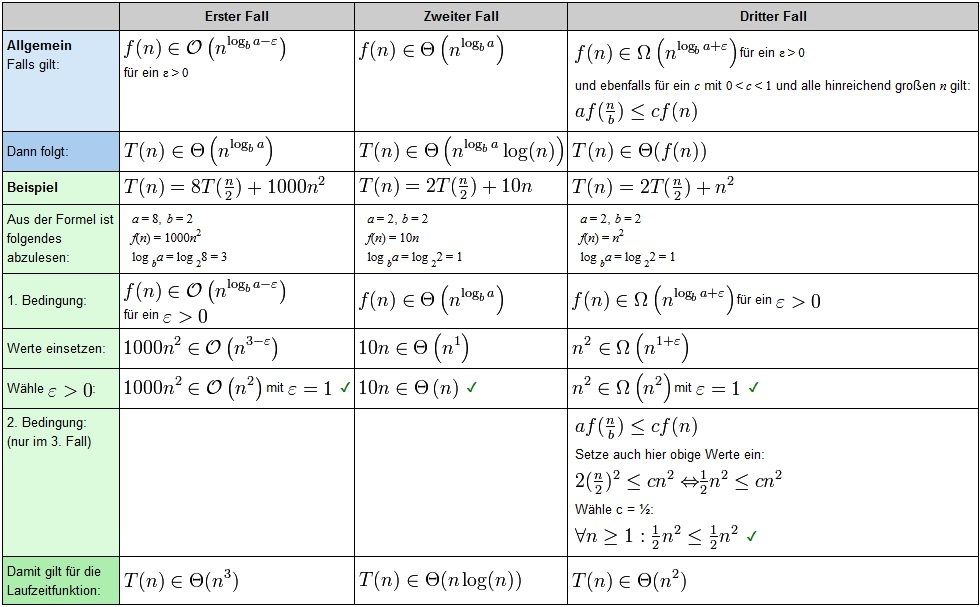
\includegraphics[scale=0.45]{masterTheorem.jpg}
\end{frame}

\begin{frame}
	\frametitle{Master-Theorem}
	\begin{block}{Ein paar Aufgaben}
		\begin{itemize}
			\item $T(n) = 9\cdot T(n/3) + n^2 + 2n + 1$
			\item $T(n) = 8\cdot T(n/2) + n\log{n}$
			\item $T(n) = 4\cdot T(n/4) + n\log{n}$
		\end{itemize}
	\end{block}
\end{frame}

\section{Automaten}

\begin{frame}
\begin{block}{Mealy Automaten}
	\begin{itemize}
		\item eine endliche Zustandsmenge Z
		\item einen Anfangszustand $z_0$ $\in$ Z
		\item ein Eingabealphabet X
		\item eine Zustandsüberführungsfunktion f: Z x X $\rightarrow$ Z
		\item ein Ausgabealphabet Y
		\item eine Ausgabefunktion g : Z x X $\rightarrow$ Y$^\ast$
	\end{itemize}	
\end{block}
\begin{block}{Moore Automaten}		
	\begin{itemize}
		\item eine endliche Zustandsmenge Z
		\item einen Anfangszustand $z_0$ $\in$ Z
		\item ein Eingabealphabet X
		\item eine Zustandsüberführungsfunktion f: Z x X $\rightarrow$ Z
		\item ein Ausgabealphabet Y
	\end{itemize} 
\end{block}
\end{frame}

\section{Akzeptoren}

\begin{frame}
	\begin{block}{Akzeptoren}
		Akzeptoren haben einen oder mehrere Akzeptierte Zustände, endet der Automat nach der Eingabe an einem dieser Zustände ist das Eingabewort akzeptiert.
		Diese Zustände werden mit einem doppelten Kreis gekennzeichnet.
		
		Mit einem solchen Akzeptor können Formale Sprachen überprüft werden.
	\end{block}
\end{frame}

\begin{frame}
	\begin{block}{Wissen}
		\begin{itemize}
			\item Nach einem britischen Gesetz von 1845 war ein Selbstmordversuch ein Kapitalverbrechen. Er war mit dem Tod durch Hängen bedroht.
			\item Das Wort Byte ist eine Verkürzung von "by eight". (sollte man Wissen)
		\end{itemize}
	\end{block}
\end{frame}

\end{document}